\subsection{Potential energy}



\begin{center}
	\includegraphics[width=\linewidth]{./lect9/pic1.png}
\end{center}

$$W=\underbrace{Fh}_{\parbox{1.5cm}{\scriptsize \centering work of \\ gravitational \\ force}}=\underbrace{mgh}_{\parbox{1.5cm}{\scriptsize \centering potential \\ energy}}$$

\paragraph{Definition} Work done by field's forces.

$$E_{height} = \vec{F}_{grav} \cdot \underbrace{\vec{x}}_{\parbox{1.5cm}{\scriptsize \centering displacement from b to a}}$$

\subparagraph{Definition} Potential energy in point $b$ relative to point $a$ is a work needed to move a body from point $a$ to $b$ without acceleration done by force opposite to field's force.

For free-falling body $E=const=mgh=\frac{mv^2}{2}+mgy$ (from conservation of the energy).

\paragraph{Conservation of energy} In a system of particles in which act mutual forces which aren't explicitly dependent on time(explicitly dependent means that constants or law itself change with time), total energy of system is conserved.

\vspace{3mm}
\centerline{ \LARGE Energy conservation $\rightleftharpoons$ symmetry in time}

\paragraph{More general results} It is convenient to talk about function of energy:

$$E = \underbrace{K}_{\parbox{1.5cm}{\scriptsize \centering  kinetic energy}} + \underbrace{U}_{\parbox{1.5cm}{\scriptsize \centering  potential \\ energy}}$$

Example of hight energy as an example:

$$U = mgh \stackrel{\parbox{2cm}{\tiny \centering  height energy equals to work of force opposite to field's forces }}{=} -F_g y = mgy$$

$$U = \left| - \vec{F}_y \right| y =  (-\hat{y} F_y)y\hat{y} = F_y y = mgy$$


Derive the equation of energy:

$$0 \stackrel{\parbox{1.5cm}{\scriptsize \centering  conservation of energy}}{=} \frac{dE}{dt} = \frac{d}{dt}\left(K+U\right) = \frac{d}{dt}\left( \frac{1}{2} mv^2 \right) + \frac{dU}{dt} = mv\frac{dv}{dt} + \frac{dU}{dy}\frac{dy}{dt} = mva + \frac{dU}{dy} \cdot v$$

We got:
$$0 = v\left( ma  +\frac{dU}{dy} \right)$$
If $m \neq 0$
$$ma = - \frac{dU}{dy}$$

This is second law of Newton we derived without usage of forces. The force is:

$$F_g = - \frac{dU}{dy}$$

In 3D we get:

$$\vec{F}_{field} = -\frac{\delta v}{\delta x}\hat{x}-\frac{\delta v}{\delta y}\hat{y}-\frac{\delta v}{\delta z}\hat{z}=-\vec{\nabla}U$$

\paragraph{Expanding treatment of force} Non-constant force in 3D:

$$\underbrace{\Delta W}_{\parbox{1cm}{\centering change in work}} = \vec{F} \cdot \Delta \vec{r} = F \Delta r \cos \alpha$$

Total work is sum of many small intervals:

$$W_{A\to B} = \int_{A}^{B} \vec{F} d\vec{r}$$

\paragraph{Example} Position of body is determined by equation $y=4x^3$. What is work of gravitation in displacement of body from $A$ to $B$.


\begin{center}
	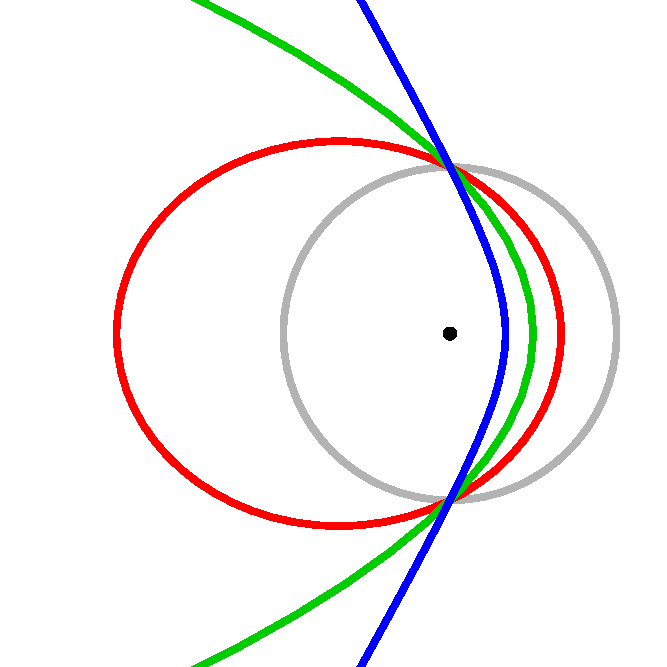
\includegraphics[width=\linewidth]{./lect9/pic2.png}
\end{center}


$$\vec{F}_G = mg(-\hat{y})$$

$$W = \int_{A}^{B} \left[ mg\left( - \hat{y} \right) \right] \cdot \left( \hat{x}dx + \hat{y}dy \right) = \int_{A}^{B} -mg dy \stackrel{\parbox{1.5cm}{\centering \scriptsize limits for x}}{=} \int_{x_A=2}^{x_B=3} \left( -mg \right) 12 x^2 dx = \left[ -mg4x^3 \right]^3_2$$

$$\frac{dy}{dx} = 12x^2 \Rightarrow dy = 12x^2 dx$$